\section{Analisis Kondisi Saat Ini}
\label{sec:analisis-kondisi-saat-ini}

Subbab ini akan membahas tentang kondisi sistem yang ada saat ini. Penulis akan mengidentifikasi masalah yang ada sekarang dan menggambarkan kondisi sistem saat ini pada \autoref{fig:current-state}. Dengan memahami bagaimana sistem saat ini beroperasi dan mengidentifikasi keterbatasan yang ada, kebutuhan fungsional dan non-fungsional sistem akan ditentukan.

\begin{figure}[htbp]
    \centering
    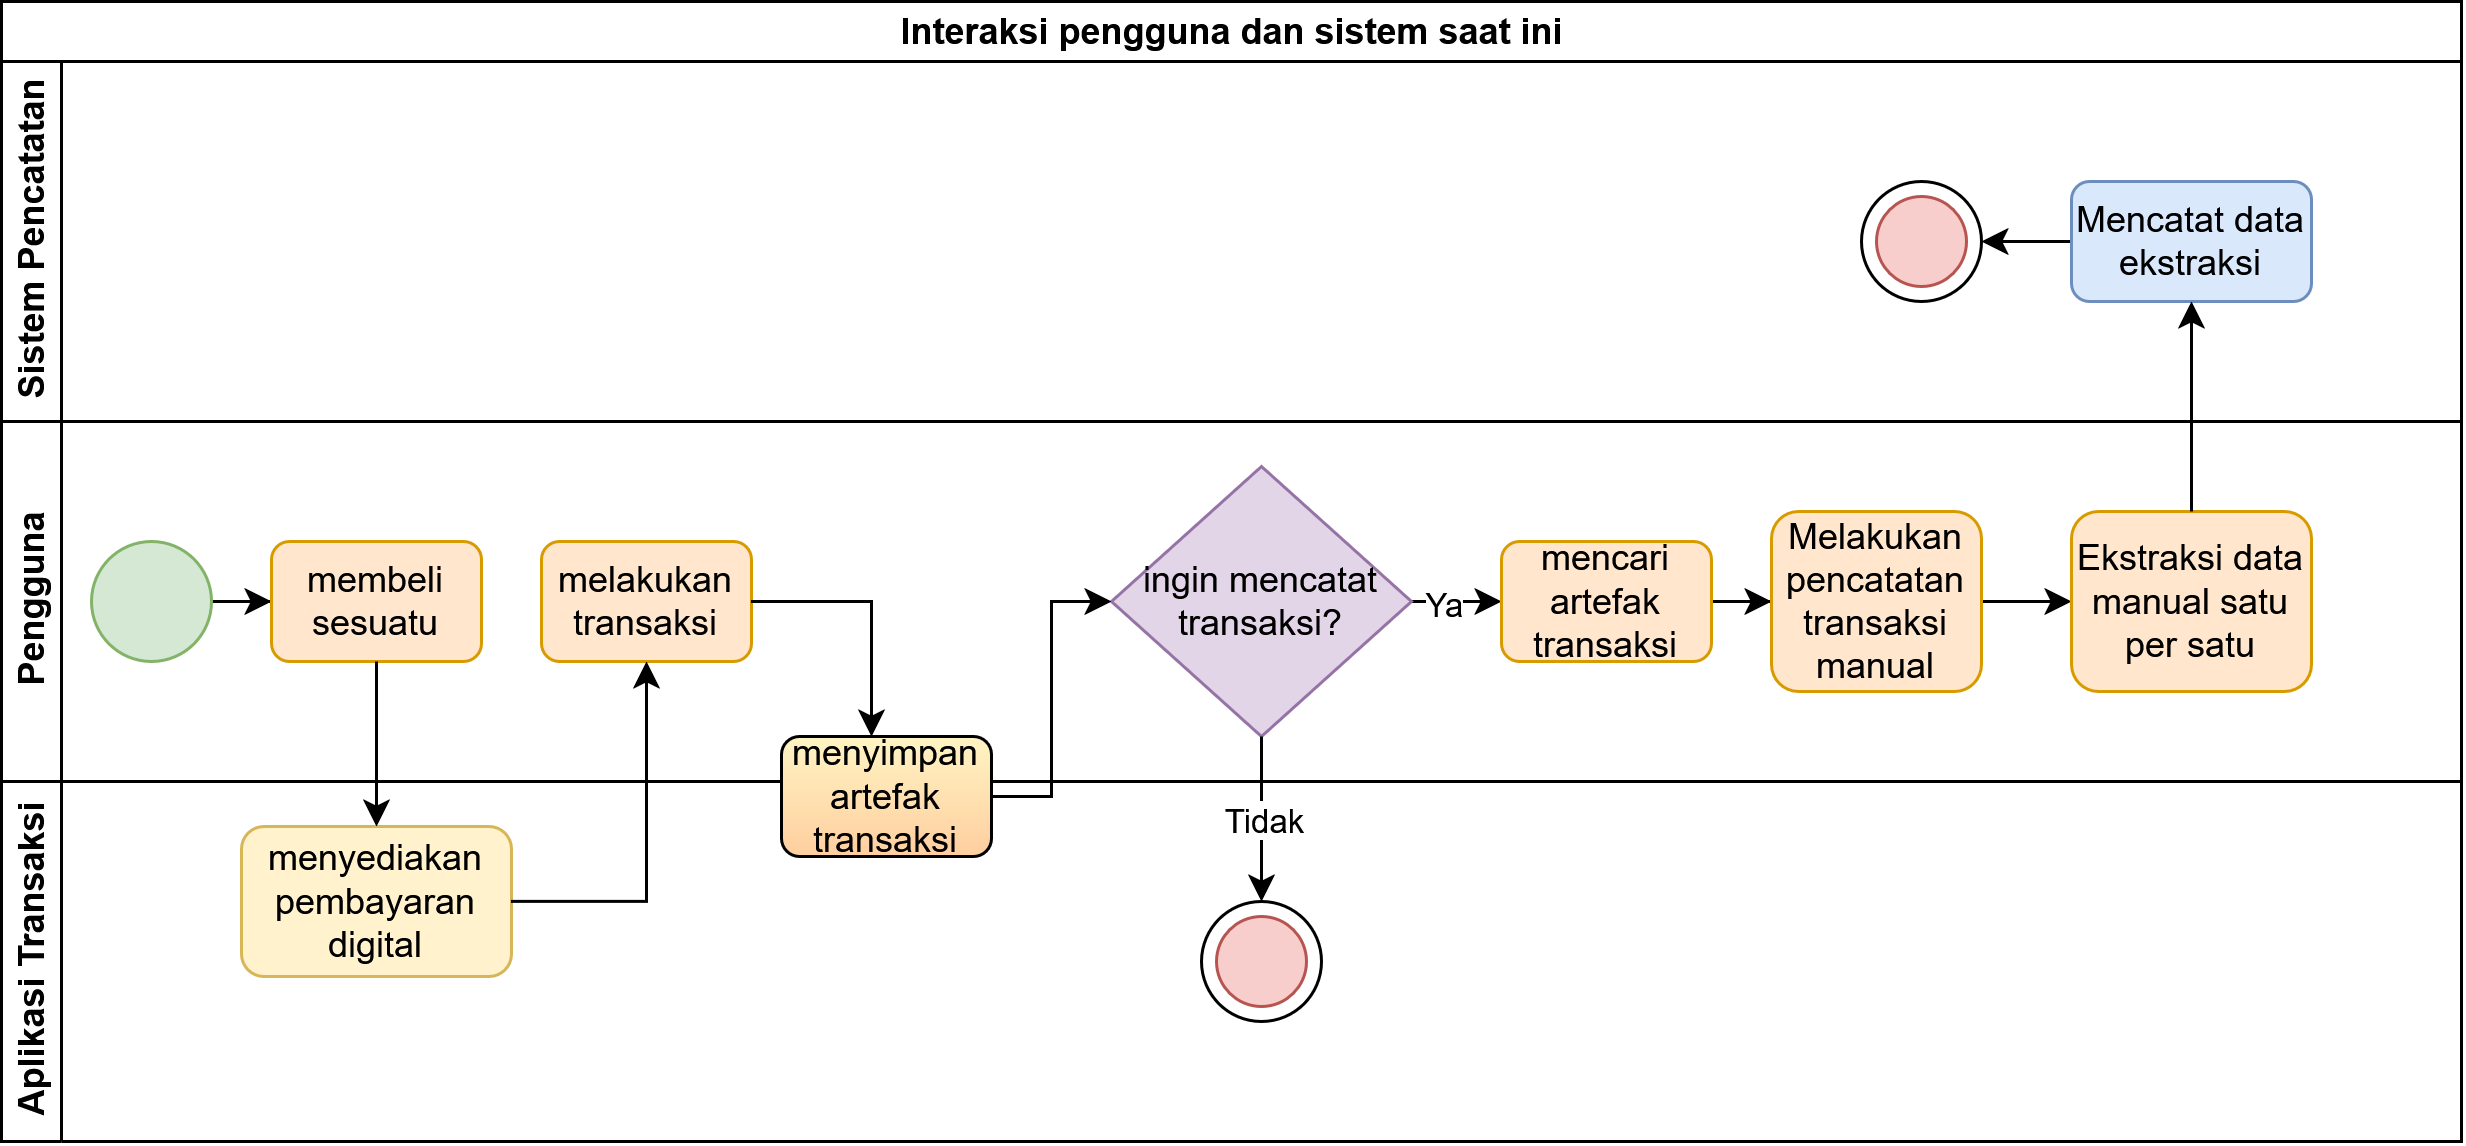
\includegraphics[width=1\textwidth]{images/current-state.png}
    \caption{BPMN kondisi saat ini}
    \label{fig:current-state}
\end{figure}

\autoref{fig:current-state} menunjukkan interaksi antara pengguna, sistem, dan aplikasi transaksi yang digunakan saat pengguna akan melakukan transaksi dan akan melakukan pencatatan transaksi tersebut. Pengguna akan melakukan transaksi melalui aplikasi transaksi saat akan membayar tagihan. Transaksi yang dilakukan dapat berupa pembayaran menggunakan QRIS atau transfer dengan artefak yang dihasilkan berupa struk pembayaran dan bukti pembayaran QRIS atau transfer. Pengguna dan aplikasi transaksi akan menyimpan artefak transaksi tersebut. Pengguna akan mencari kembali artefak transaksi tersebut saat akan melakukan pencatatan transaksi dan melakukan ekstraksi data secara manual dan mencatat data tersebut ke dalam aplikasi pencatatan keuangan yang dimiliki.

\begin{figure}[htbp]
    \centering
    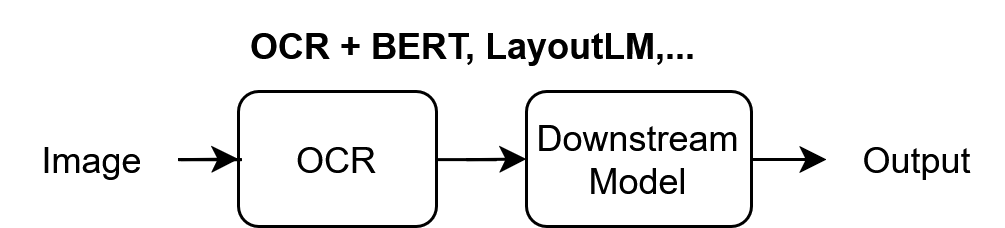
\includegraphics[width=0.8\textwidth]{images/non-donut-pipeline.png}
    \caption{\emph{Pipeline} sistem yang digunakan umumnya}
    \label{fig:non-donut-pipeline}
\end{figure}

\autoref{fig:non-donut-pipeline} menunjukkan alternatif yang umumnya ditemui jika pengguna tidak perlu melakukan ekstraksi data secara manual. Pengguna hanya perlu melakukan upload kemudian sistem akan melakukan ekstraksi data dari artefak yang diunggah. Sistem akan melakukan ekstraksi data dengan menggunakan \ocr{} untuk mendapatkan teks dari artefak yang diunggah. Setelah itu, sistem akan melakukan ekstraksi data dari teks yang telah didapatkan dengan menggunakan model yang telah dilatih sebelumnya. Hasil ekstraksi data akan disimpan ke dalam aplikasi pencatatan keuangan yang dimiliki pengguna.

